\begin{figure}[htp]
    \centering
    \resizebox{.5\textwidth}{!}{
    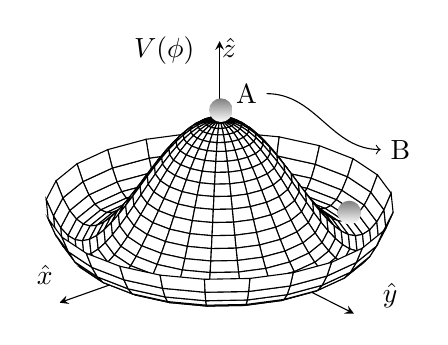
\begin{tikzpicture}
      \begin{axis}[
          axis lines=center,
          view={140}{25},
          axis equal,
          domain=0:360,
          y domain=0:1.25,
          xmax=1.5,ymax=1.5,zmin=0,zmax=1.5,
          x label style={at={(axis description cs:0.18,0.29)},anchor=north},
          y label style={at={(axis description cs:0.82,0.25)},anchor=north},
          z label style={at={(axis description cs:0.44,0.8)},anchor=north},
          xlabel = $\hat{x}$,
          ylabel=$\hat{y}$,
          zlabel=$V(\phi)\quad \hat{z}$,
          ticks=none,
          clip bounding box=upper bound
        ]
    
        \addplot3 [surf, shader=flat, draw=black, fill=white, z buffer=sort] ({sin(x)*y}, {cos(x)*y}, {(y^2-1)^2});
      \end{axis}
      \shade (3.47,3.5) circle [radius=0.15cm];
      \shade (5.1,2.2) circle [radius=0.15cm];
      \node[anchor=east] at (4.05,3.71) (text) {A};
      \node[anchor=west] at (5.5,3.0) (description) {B};
      \draw (description) edge[out=180,in=0,<-] (text);
    \end{tikzpicture}
    }
    \caption{Illustration of the Higgs potential. There is an infinite number of ground states. At point A, the global symmetry is unbroken. At point B, a local minimum is chosen and spontaneous symmetry breaking occurs. This figure is from Ref.~\cite{higgspotential}.}
    \label{fig:Higgspotential}
\end{figure}